\documentclass[aspectratio=169,11pt]{beamer}

% Shared style (ib-tutorials.sty at the repo root).
\makeatletter\def\input@path{{./}{../}}\makeatother
\usepackage{ib-tutorials}

\usepackage[utf8]{inputenc}
\usepackage{amsmath,amssymb}
\usepackage{booktabs}
\usepackage{array}
\newcolumntype{L}[1]{>{\raggedright\arraybackslash}p{#1}}
\usepackage{graphicx}
\graphicspath{{../pictures/3-ibamr-fundamentals/}{pictures/3-ibamr-fundamentals/}}
\usepackage{xcolor}
\usepackage{listings}
\usepackage{tikz}
\usetikzlibrary{arrows.meta,positioning,shapes.geometric,fit,calc}
\usepackage{hyperref}

\newcommand{\sourcecredit}[1]{\vfill\hfill{\tiny\textcolor{DarkGray}{#1}}}

\lstset{
  basicstyle=\ttfamily\scriptsize\color{BlackGray},
  keywordstyle=\color{NavyBlue}\bfseries,
  commentstyle=\color{DarkGray}\itshape,
  stringstyle=\color{OliveGreen},
  showstringspaces=false,
  columns=fullflexible,
  keepspaces=true,
  frame=single,
  framerule=0.4pt,
  rulecolor=\color{LightGray},
  backgroundcolor=\color{LightGray!30},
  xleftmargin=0.25em,
  xrightmargin=0.25em
}
\lstdefinestyle{shell}{morecomment=[l]{\#}}
\lstdefinestyle{input}{morecomment=[l]{//}}
\lstdefinestyle{matlab}{morecomment=[l]{\%}}
\lstdefinestyle{data}{}
\lstdefinestyle{tiny}{basicstyle=\ttfamily\tiny\color{BlackGray}}

\title[Structure files]{Structure files}
\subtitle{How an immersed structure is described to IBAMR: vertices, springs, beams, targets and the rest}
\author[Miller]{Laura A. Miller}
\institute[UArizona]{Department of Mathematics, University of Arizona}
\date{Using IB Software \textbullet\ Part III \textbullet\ Chapter 6}

\begin{document}

% 1
\begin{frame}[plain]
\maketutorialtitlepanel{%
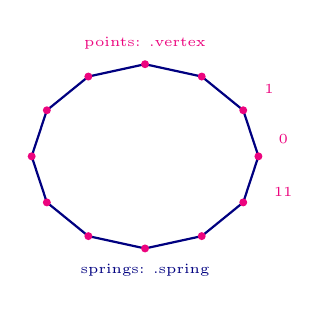
\begin{tikzpicture}[scale=0.9]
  \foreach \i in {0,...,11}{
    \coordinate (p\i) at ({1.6*cos(30*\i)},{1.3*sin(30*\i)});}
  \foreach \i [evaluate=\i as \j using {int(mod(\i+1,12))}] in {0,...,11}{
    \draw[NavyBlue,thick] (p\i) -- (p\j);}
  \foreach \i in {0,...,11}{\fill[RubineRed] (p\i) circle (1.6pt);}
  \node[font=\tiny,text=RubineRed] at (1.95,0.25) {0};
  \node[font=\tiny,text=RubineRed] at (1.75,0.95) {1};
  \node[font=\tiny,text=RubineRed] at (1.95,-0.5) {11};
  \node[font=\tiny,text=NavyBlue] at (0,-1.6) {springs: \code{.spring}};
  \node[font=\tiny,text=RubineRed] at (0,1.6) {points: \code{.vertex}};
\end{tikzpicture}}
\end{frame}

% 2
\begin{frame}{Learning goals}
\small By the end of this chapter you should be able to:
\begin{enumerate}
  \item name every structure file that IBAMR's standard initializer reads, say what each one adds to the model, and read the ones used in this series (\code{.vertex}, \code{.spring}, \code{.beam}, \code{.target}) line by line;
  \item say how points are numbered, what the stiffness numbers in the files mean and in what units, and what is required and what is optional in each line;
  \item connect the files to the input file (\code{structure\_names}, \code{level\_number}, the \code{uniform\_*} and \code{enable\_*} keys) and to the log, which reports what was read;
  \item write a generator script (MATLAB or Python) that produces the files for a new structure, and check the result before running;
  \item recognize the errors IBAMR prints for a malformed file, and the mistakes it does not catch.
\end{enumerate}
\vspace{2mm}
\begin{punchbox}
\small Every format in this chapter was checked against the reader in IBAMR 0.19.0 (\code{src/IB/IBStandardInitializer.cpp}) and against runs of the examples with deliberately broken files. Where the official header comment and the code disagree, the code wins, and the slide says so.
\end{punchbox}
\end{frame}

% 3
\begin{frame}{Learning IBAMR: where to look things up}
\begin{itemize}
  \item The code and its examples: \url{https://github.com/IBAMR/IBAMR}. The examples folder is the best reference for what each file and key does in practice (chapter 15).
  \item The web site and documentation index: \url{https://ibamr.github.io} and \url{https://ibamr.github.io/docs}. The old per-class pages (\code{ibamr.github.io/IBAMR/ibamr/html/}) no longer exist.
  \item The \al{file formats are documented in the header} \code{include/ibamr/IBStandardInitializer.h} of the source tree, which autoibamr leaves unpacked under \code{tmp/unpack/IBAMR-<version>/}. Open it next to this chapter.
\end{itemize}
\vspace{2mm}
\begin{punchbox}
\small When a slide here and the header comment disagree, trust the slide: the comment says the rest length of a spring is optional, and the reader stops with an error when it is missing (slide 12, tested).
\end{punchbox}
\end{frame}

% 3b
\begin{frame}{Learning IBAMR: the community and the method}
\begin{itemize}
  \item The wiki and its FAQ: \url{https://github.com/IBAMR/IBAMR/wiki} (partly dated: it predates CMake builds).
  \item Questions: the IBAMR Users Google group, \url{https://groups.google.com/g/ibamr-users}, and GitHub Discussions, \url{https://github.com/IBAMR/IBAMR/discussions}. Development discussion is on the developers' group, \code{ibamr-dev@googlegroups.com}.
  \item The method: Peskin's page, \url{https://math.nyu.edu/~peskin/}, and the 2002 Acta Numerica paper (chapter 5).
\end{itemize}
\vspace{2mm}
\small The 2015 lecture pointed to the Google Code site (\code{ibamr.googlecode.com}) for the class documentation, the source browser and the file-format page; Google Code closed in 2016. The 2020 lecture's class-documentation link returns 404 today. Links checked October 2026.
\end{frame}

% 4
\begin{frame}{Two kinds of input}
\begin{columns}[T,onlytextwidth]
\begin{column}{0.5\textwidth}
\al{The input file}, \code{input2d} or \code{input3d} (chapters 3 and 7):
\begin{itemize}
  \item physical parameters: density, viscosity, the box, boundary conditions;
  \item numerical parameters: the grid levels, \code{DT}, the run length, output intervals;
  \item and the block that names the structures.
\end{itemize}
\end{column}
\begin{column}{0.48\textwidth}
\al{The structure files}, one set per structure, named \code{<name>.<extension>}:
\begin{itemize}
  \item the \al{initial positions} of the points (\code{.vertex}), the only required file;
  \item the \al{elastic elements} that join or hold them: springs, beams, target points, and the less common ones.
\end{itemize}
\end{column}
\end{columns}
\vspace{2mm}
\begin{punchbox}
\small The structure files say what the structure \emph{is}; the input file says where it goes, on which grid level, and lets you override its stiffnesses without rewriting it (slide 24). The program (\code{main.cpp}) usually knows nothing about either: it reads both at start-up through \code{IBStandardInitializer}.
\end{punchbox}
\small The files are plain text. You write them with a script (slides 29--33) and read them with any editor; the examples in this series ship both the files and the scripts that made them.
\end{frame}

% 5
\begin{frame}{The files IBAMR reads}
\scriptsize
\begin{tabular}{@{}L{0.09\textwidth}L{0.4\textwidth}L{0.11\textwidth}L{0.28\textwidth}@{}}
\toprule
File & What it specifies & Required? & Used in\\
\midrule
\code{.vertex} & the initial position of every point & \al{yes} & every example\\
\code{.spring} & linear or nonlinear springs between pairs of points & no & IB/01--04, 06, 07\\
\code{.beam} & bending resistance for triples of points, with an optional preferred curvature & no & IB/02, 03, 07; chapter 10\\
\code{.target} & points tethered to their initial position (or to a moving target) by stiff springs & no & IB/02--04, 07, 08; chapter 9a\\
\code{.xspring} & ``crosslink'' springs that may join points of different structures (global indices) & no & chapter 9a\\
\code{.anchor} & points fixed in place that exchange nothing with the fluid & no & slide 18\\
\code{.mass} & extra mass on points (penalty immersed boundary) & no & chapter 13\\
\code{.rod}, \code{.director} & Kirchhoff rods that resist bending and twisting, and their material frames & no & slide 21; chapter 15\\
\code{.inst} & flow meters built from points & no & slide 22; chapter 15\\
\code{.source} & fluid sources and sinks attached to points & no & slide 22; chapter 15\\
\bottomrule
\end{tabular}
\vspace{2mm}
\small The extensions are fixed; the base name is yours and goes in \code{structure\_names}.
\end{frame}

% 5b
\begin{frame}{What the table does not say}
\begin{itemize}
  \item Every optional file that is absent is \al{silently skipped}, with one line in the log (slide 25). A structure with no \code{.spring}, \code{.beam} or \code{.target} file is a cloud of free points that the fluid carries along, and nothing on the screen says so.
  \item The files describe \al{elements}, not materials: a spring is two points and two numbers, a beam three points and one number. Chapters 8a and 8b say how to choose the numbers from a material and a size; chapter 9b how to make them depend on time.
  \item One structure can have all of the files at once (the leaf has four), and the same point can be in several elements: a point can be the end of two springs, the middle of a beam and a target point, as the leaf's points 50 and 51 are.
  \item IBFE structures are different: a finite element mesh file (MSH or ExodusII) replaces this whole set, and the elasticity is a function in the program (Part IV). The two can be mixed in one run.
\end{itemize}
\end{frame}

% 6
\begin{frame}[fragile]{How IBAMR finds the files}
\begin{columns}[T,onlytextwidth]
\begin{column}{0.48\textwidth}
\begin{lstlisting}[style=input]
IBStandardInitializer {
   max_levels = MAX_LEVELS
   structure_names = "leaf_512"
   leaf_512 {
      level_number = MAX_LEVELS - 1
   }
}
\end{lstlisting}
\small Several structures: \code{structure\_names = "plate2d\_left\_512", "plate2d\_rght\_512"}, each with a sub-block (IB/07; chapter 9a).
\end{column}
\begin{column}{0.5\textwidth}
\small
\begin{itemize}
  \item \code{structure\_names} lists the base names; for each, IBAMR opens \code{<name>.vertex} in the \al{working directory} (where you run \code{mpirun}), then tries every other extension.
  \item Each structure has its own sub-block with its \code{level\_number}: the grid level it lives on, almost always the finest, \code{MAX\_LEVELS - 1} (chapter 5).
  \item The program never names the files: \code{main.cpp} only passes the \code{IBStandardInitializer} block to the initializer.
\end{itemize}
\end{column}
\end{columns}
\vspace{1mm}
\begin{punchbox}
\small The base name is also the name of the mesh in VisIt (\code{leaf\_512\_mesh}) and the prefix of the restart data, so choose it before you generate the files and keep it. The older key \code{base\_filenames}, one list per level, still works but is not used in this series.
\end{punchbox}
\end{frame}

% 7
\begin{frame}[fragile]{The \code{.vertex} file}
\begin{columns}[T,onlytextwidth]
\begin{column}{0.5\textwidth}
\begin{lstlisting}[style=data]
N                 # number of points in the file
x_0  y_0          # position of point 0
x_1  y_1          # position of point 1
...
x_{N-1}  y_{N-1}  # position of point N-1
\end{lstlisting}
\small In 3D each line has three numbers, \code{x y z}.
\end{column}
\begin{column}{0.48\textwidth}
\small The rubber band's file begins
\begin{lstlisting}[style=tiny]
644
0.0000000000000000e+00 1.0000000000000001e-01
1.0244161346221071e-03 9.9995240574191152e-02
2.0487347565924115e-03 9.9980962749807278e-02
3.0728583625411962e-03 9.9957167885933298e-02
\end{lstlisting}
and continues for 644 lines: 644 points of the band, in meters, each about $\Delta x/2$ from the next.
\end{column}
\end{columns}
\vspace{2mm}
\begin{itemize}
  \item The first line is the \al{count} $N$; then exactly $N$ lines of coordinates, in the units of the input file (meters here).
  \item The \al{index of a point is its line number}, counting from 0: the first coordinate line is point 0, the last is point $N-1$. Nothing in the file says ``point 7''; its place does.
\end{itemize}
\end{frame}

% 7b
\begin{frame}{Reading a \code{.vertex} file}
\begin{itemize}
  \item Text after a \code{\#}, \code{\%} or \code{!} on a coordinate line is ignored, so you may annotate a \code{.vertex} file. A line that holds only a comment is an error (slide 26).
  \item \code{posn\_shift} and \code{length\_scale\_factor} in the structure's input sub-block move and scale the points as they are read, without rewriting the file (slide 24).
  \item The order of the lines is the geometry's own order: for a curve, walk along it; for a ring, go around once; for several rings (the bristles of IB/04), one ring after another. The \code{.spring} and \code{.beam} files refer to these line numbers, so the generator that writes the points must be the one that writes the elements.
  \item Coordinates are written with 17 significant digits (\code{\%1.16e}) so that the file holds the exact double; three decimals would do for the physics but would make the Python and MATLAB generators disagree on the last digit (Appendix A compares them).
  \item A 3D \code{.vertex} file for a 2D run, or the reverse, fails at once: the reader expects exactly \code{NDIM} numbers per line.
\end{itemize}
\end{frame}

% 8
\begin{frame}{Point numbers: local and global}
\footnotesize
\begin{itemize}
  \item Within one structure, points are numbered \al{0 to $N-1$} by their order in the \code{.vertex} file, and the \code{.spring}, \code{.beam}, \code{.target}, \code{.anchor} and \code{.mass} files refer to these \al{local} numbers.
  \item When the input lists several structures, IBAMR numbers all their points together in the order of \code{structure\_names}: the first structure's points keep their numbers, the second structure's are offset by the first's count, and so on. These are the \al{global} indices.
  \item Only one file in the standard set uses global indices: \code{.xspring}, because a crosslink spring may join two structures. The program can ask for a structure's range with \code{getLagrangianStructureIndexRange} (IB/07).
  \item Changing the order in \code{structure\_names} changes every global index; the local files do not change.
\end{itemize}
\vspace{1mm}
\begin{punchbox}
\small IBAMR counts from 0; MATLAB and IB2d count from 1. A \code{.spring} file written with MATLAB's loop variable as the index is off by one, and IBAMR stops at the first index equal to $N$: \code{vertex index 644 is out of range} (slide 26). The generators in this series loop \code{for s = 0:npts-1} for exactly this reason.
\end{punchbox}
\small Chapter 9a uses local and global indices side by side for the two plates of IB/07 (points 0--102 and 103--205).
\end{frame}

% 9
\begin{frame}[fragile]{The \code{.spring} file}
\begin{columns}[T,onlytextwidth]
\begin{column}{0.5\textwidth}
\begin{lstlisting}[style=data]
M                          # number of springs
i_0  j_0  kappa_0  L_0  [fcn_0  [p_1 p_2 ...]]
i_1  j_1  kappa_1  L_1  [fcn_1  [...]]
...
\end{lstlisting}
\small Each line: the two points it joins, its \al{stiffness} $\kappa$, its \al{rest length} $L$, and optionally a force-function index (slide 14) and extra parameters for that function.
\end{column}
\begin{column}{0.48\textwidth}
\small The rubber band's file:
\begin{lstlisting}[style=tiny]
644
0 1 2.0499156670236122e+06 9.7564989241919039e-04
1 2 2.0499156670236122e+06 9.7564989241919039e-04
...
642 643 2.0499156670236122e+06 9.7564989241919039e-04
643 0 2.0499156670236122e+06 9.7564989241919039e-04
\end{lstlisting}
644 springs for 644 points: each joins a point to the next, and the last one closes the ring.
\end{column}
\end{columns}
\vspace{2mm}
\small The force of a spring of current length $R$ is $\kappa\,(R - L)$ along the line between its points, pulling when stretched and pushing when compressed, with equal and opposite forces on the two ends (\code{default\_spring\_force} in \code{IBSpringForceFunctions.h}).
\end{frame}

% 10
\begin{frame}{Springs: what else to know}
\begin{itemize}
  \item Any number of springs may meet at a point; a point may also have none. A network of springs (a sheet, a lattice, the cross-braced wing of chapter 9a) is just a longer \code{.spring} file.
  \item The lower of the two indices is the spring's ``master'' point, the one whose data holds the spring; IB/06 changes rest lengths through it.
  \item A spring with $\kappa = 0$ does nothing but is still drawn by VisIt (slide 35): the header suggests a zero-stiffness \code{.spring} file for structures that have no springs, so that they can be plotted as lines.
  \item A spring whose rest length is shorter than the points' distance starts under tension; longer, under compression. The rubber band starts stretched (an ellipse with the rest lengths of a circle), which is what makes it move.
  \item Springs do not resist bending: a chain of springs folds freely, as IB/06 shows. Beams add that (slide 16).
\end{itemize}
\end{frame}

% 11
\begin{frame}{What is required on a spring line}
\begin{itemize}
  \item The header comment in \code{IBStandardInitializer.h} says the rest length and the function index are optional, with defaults 0 and 0.
  \item \al{The rest length is not optional}: a file with only \code{i j kappa} on each line stops IBAMR with \code{Invalid entry in input file encountered on line 2 of file rubber\_band\_512.spring} (tested with 0.19.0). The function index is optional.
  \item Four numbers per line, then: two indices, $\kappa$, $L$. Anything after the required and optional numbers is ignored, which is why a trailing \code{// spring} on each line passes (slide 26). Do not rely on it.
\end{itemize}
\vspace{2mm}
\begin{punchbox}
\small If you want a zero rest length (a spring that pulls its ends together until they meet), write the 0: \code{i j kappa 0.0}.
\end{punchbox}
\end{frame}

% 12
\begin{frame}{The closing spring}
\begin{columns}[T,onlytextwidth]
\begin{column}{0.55\textwidth}
\begin{itemize}
  \item A ring of $N$ points needs $N$ springs, the last one joining point $N-1$ back to point 0.
  \item The UNC course's generator wrote \code{npts-1} springs with the loop \code{for s = 0:npts-2}, so its band had a gap: 643 springs for 644 points. The 2022 version and IB/01 write 644, with \code{mod(s+1, npts)} as the second index of the last spring.
  \item The 2018 and 2020 lectures showed the 643-spring file as the example output; the gap went unnoticed for years because the band still looked round.
\end{itemize}
\end{column}
\begin{column}{0.43\textwidth}
\begin{punchbox}
\small A missing closing spring is invisible in the files and in the log (644 points, 643 edges: both numbers look fine). It shows in VisIt as a gap in the mesh line, and in the physics as a band that does not hold its pressure. Check the count: a closed curve has as many springs as points.
\end{punchbox}
\end{column}
\end{columns}
\end{frame}

% 13
\begin{frame}[fragile]{Spring force functions}
\small The fifth number on a spring line, the \al{function index}, chooses how the force depends on the length. Index 0 (the default) is the linear spring $F = \kappa\,(R - L)$. A program can register its own functions under other indices:
\begin{lstlisting}[style=tiny]
// in main.cpp, before the run (chapter 9b)
double my_force(double R, const double* params, int lag_mastr_idx, int lag_slave_idx)
{   // params[0] = kappa, params[1] = L, params[2..] = the extras on the spring's line
    return params[0] * (R - params[1]) * (R - params[1]);
}
...
ib_force_fcn->registerSpringForceFunction(1, &my_force);
\end{lstlisting}
A line \code{i j kappa L 1 a b} in the \code{.spring} file then uses \code{my\_force} with \code{params = \{kappa, L, a, b\}}.
\end{frame}

% 14
\begin{frame}{Spring force functions: how they are used}
\begin{itemize}
  \item The extra parameters are read from the line after the index, as many as there are (\code{while (line\_stream >> param)}), and stored with the spring.
  \item \code{uniform\_spring\_force\_fcn\_idx} in the input sub-block sets the index for every spring of a structure without rewriting the file (slide 24).
  \item The function receives the two point indices too, so it can look up anything about them (a stiffness that varies along the body, say). Register functions before the time loop starts.
  \item A derivative function can be registered alongside (\code{registerSpringForceFunction(idx, \&f, \&df)}); IBAMR uses it for the implicit solvers and ignores it in the explicit ones used here.
  \item Chapter 9b builds a muscle-like spring this way; IB/06 changes the rest length of linear springs in time instead, which needs no new function.
\end{itemize}
\end{frame}

% 15
\begin{frame}{What the stiffness numbers mean, and their units}
\small The generators of this series write
\[
\kappa_{\text{file}} = \frac{K}{\Delta s} \quad(\text{springs and targets}), \qquad
\kappa_{b,\text{file}} = \frac{EI}{\Delta s^3} \quad(\text{beams}),
\]
where $\Delta s$ is the point spacing, $K$ is the structure's stretching stiffness (its tension per unit strain, in newtons) and $EI$ its bending stiffness (in N\,m$^2$). Why:
\begin{itemize}
  \item A spring between neighbors $\Delta s$ apart, stretched by $R - L = \varepsilon\,\Delta s$ (strain $\varepsilon$), pulls with $\kappa_{\text{file}}(R - L) = K\varepsilon$: the tension of the material, independent of how finely it is discretized.
  \item A beam's force uses the second difference $X_{i-1} - 2X_i + X_{i+1} \approx \Delta s^2\,\partial_s^2 X$; dividing $EI$ by $\Delta s^3$ makes the bending moment per point come out as $EI$ times the curvature, again independent of the spacing.
  \item A target point's force $\kappa_{\text{file}}(X_{\text{target}} - X)$ is then the force per point of a tether with stiffness $K$ per unit length.
\end{itemize}
\end{frame}

% 15b
\begin{frame}{The stiffness numbers: consequences}
\begin{itemize}
  \item The file numbers change when you refine the structure, and that is why the generators, not the files, hold the physical constants: \code{kappa\_spring = 2.0e3} (N) in IB/01's script becomes $2.05\times10^6$ N/m in the file, for $\Delta s = 9.8\times10^{-4}$ m.
  \item Two structures with the same $K$ but different point spacings have different file numbers; comparing stiffnesses across files is meaningless without $\Delta s$.
  \item The older lectures never said what the file $\kappa$ was; the 2013 generator comments called $\kappa_{\text{spring}}$ a ``spring constant (Newton)'' without the division. The expression they used, \code{kappa\_spring*ds/(ds\textasciicircum 2)}, is $K/\Delta s$ written in two steps.
  \item In dimensionless inputs (the IBFE examples, most of IB2d's) the same scaling holds with dimensionless $K$ and $EI$. Chapter 8b shows how to choose $K$ and $EI$ from a real material, and how they scale.
\end{itemize}
\vspace{2mm}
\begin{punchbox}
\small Rule: keep $K$ and $EI$ in the generator, compute $\Delta s$ from the grid, and let the script do the division.
\end{punchbox}
\end{frame}

% 16
\begin{frame}[fragile]{The \code{.beam} file}
\begin{columns}[T,onlytextwidth]
\begin{column}{0.5\textwidth}
\begin{lstlisting}[style=data]
M                              # number of beams
i_0  j_0  k_0  kappa_0  [Cx_0  Cy_0  [Cz_0]]
i_1  j_1  k_1  kappa_1  [Cx_1  Cy_1  [Cz_1]]
...
\end{lstlisting}
\small Each line: three consecutive points, a \al{bending rigidity} $\kappa_b$, and optionally a preferred curvature vector $\mathbf{C}$ with as many components as the problem has dimensions.
\end{column}
\begin{column}{0.48\textwidth}
\small The leaf's file (IB/03):
\begin{lstlisting}[style=tiny]
101
0 1 2 5.3060400000000009e+06
1 2 3 5.3060400000000009e+06
...
100 101 102 5.3060400000000009e+06
\end{lstlisting}
101 beams for 103 points: one per interior point.
\end{column}
\end{columns}
\vspace{2mm}
\small The beam resists the second difference $\mathbf{X}_i - 2\mathbf{X}_j + \mathbf{X}_k$: its energy is $\tfrac{1}{2}\kappa_b\,|\mathbf{X}_i - 2\mathbf{X}_j + \mathbf{X}_k - \mathbf{C}|^2$, and the force on each of the three points is minus the gradient of that energy, with the stencil $(1, -2, 1)$.
\end{frame}

% 16b
\begin{frame}{Beams: what else to know}
\begin{itemize}
  \item The \al{middle index $j$ is the master} point and must be an interior point of the triple; $N$ points in a line give $N-2$ beams, one per interior point, and a ring of $N$ points gives $N$ beams (the two that wrap around included).
  \item With no curvature given, $\mathbf{C} = 0$: the beam is straight at rest. A curvature vector makes a curved rest shape, which is how chapter 10 makes a jellyfish bell and changes it in time; the vector is the preferred value of $\mathbf{X}_i - 2\mathbf{X}_j + \mathbf{X}_k$, so it scales with $\Delta s^2$.
  \item Beams and springs on the same points are the usual pair: springs keep the length, beams the shape. The leaf has both; the bristles of IB/04 have neither, only targets.
  \item \code{uniform\_beam\_bend\_rigidity} and \code{uniform\_beam\_curvature} override the file (slide 24).
  \item Beams are the fourth file that VisIt does not draw (slide 35): a structure with beams only shows as points.
\end{itemize}
\end{frame}

% 17
\begin{frame}[fragile]{The \code{.target} file}
\begin{columns}[T,onlytextwidth]
\begin{column}{0.5\textwidth}
\begin{lstlisting}[style=data]
M                    # number of target points
i_0  kappa_0  [eta_0]
i_1  kappa_1  [eta_1]
...
\end{lstlisting}
\small Each line: a point index, the \al{tether stiffness} $\kappa$, and optionally a \al{damping coefficient} $\eta$ (0 if absent).
\end{column}
\begin{column}{0.48\textwidth}
\small The leaf's two target points, and the first lines of the bristles' file, where every point is a target:
\begin{lstlisting}[style=tiny]
2
50 3.0600000000000004e+04
51 3.0600000000000004e+04
\end{lstlisting}
\begin{lstlisting}[style=tiny]
297
0 4.0960000000000000e+06
1 4.0960000000000000e+06
\end{lstlisting}
\end{column}
\end{columns}
\vspace{2mm}
\small A target point is tethered to a \al{target position} by a linear spring of zero rest length and, if $\eta > 0$, a dashpot: force $\kappa\,(\mathbf{X}_{\text{target}} - \mathbf{X}) - \eta\,\mathbf{U}$. The target position starts at the point's initial position.
\end{frame}

% 17b
\begin{frame}{Target points: what else to know}
\begin{itemize}
  \item A target point approximately pins its point: the stiffer $\kappa$, the smaller the lag, and the smaller the stable time step (chapter 5, slide 27). The lag is the force divided by $\kappa$, which the READMEs of IB/03, 04 and 07 report.
  \item The program may move the target positions during the run, which is how prescribed motion is done (IB/04, IB/07, IB/08; chapter 9a). The file only says which points are tethered and how stiffly; the motion is code.
  \item The damping $\eta$ dissipates the oscillation of a point about its target; the 2013 lecture lost its symbol in a font change, and the course files never used it. With $\eta = 0$ the target is a pure spring, a Kelvin--Voigt element with the dashpot removed.
  \item Listing a point twice gives the warning \code{Duplicate target point node}; \code{uniform\_target\_stiffness} and \code{uniform\_target\_damping} override the file (slide 24).
  \item Targets are not drawn by VisIt either, but the points they hold are: a tethered structure looks like any other.
\end{itemize}
\end{frame}

% 18
\begin{frame}[fragile]{The \code{.anchor} file}
\begin{columns}[T,onlytextwidth]
\begin{column}{0.4\textwidth}
\begin{lstlisting}[style=data]
M        # number of anchor points
i_0
i_1
...
\end{lstlisting}
\small One index per line.
\end{column}
\begin{column}{0.58\textwidth}
\footnotesize An \al{anchor point} neither spreads force to the fluid nor interpolates velocity from it: it is literally anchored where it starts, whatever the fluid does.
\begin{itemize}
  \item Anchor points are not target points. A target point is tethered by a spring and moves a little; an anchor point does not move at all and exerts no force of its own. A spring from a structure to an anchor point behaves like a spring to a fixed wall.
  \item Use them for the fixed end of a tether, for a support that should not feel the flow, or to hold the end of a filament exactly.
  \item \code{enable\_anchor\_points = FALSE} in the input sub-block turns them back into ordinary points without editing the file.
\end{itemize}
\end{column}
\end{columns}
\vspace{1mm}
\begin{punchbox}
\small Think of target points as tethered to invisible anchor points: the 2020 lecture's phrase, and a good way to keep the two apart.
\end{punchbox}
\end{frame}

% 19
\begin{frame}[fragile]{The \code{.mass} file}
\begin{columns}[T,onlytextwidth]
\begin{column}{0.5\textwidth}
\begin{lstlisting}[style=data]
M                    # number of mass points
i_0  mass_0  kappa_0
i_1  mass_1  kappa_1
...
\end{lstlisting}
\small Each line: a point index, the \al{mass} carried by that point, and the \al{penalty stiffness} of the spring that ties the point to its massive copy.
\end{column}
\begin{column}{0.48\textwidth}
\small
\begin{itemize}
  \item The immersed boundary points themselves are massless: they move with the fluid.
  \item To give a structure mass, IBAMR's \al{penalty immersed boundary} method attaches to each listed point a ``ghost'' particle with the given mass, which moves by Newton's laws (gravity included), and ties the two with a stiff spring of zero rest length.
\end{itemize}
\end{column}
\end{columns}
\end{frame}

% 19b
\begin{frame}{Mass points: what else to know}
\begin{itemize}
  \item The penalty stiffness plays the same role as a target stiffness: stiffer means the point follows its massive copy more closely and the time step must be smaller.
  \item The mass is per point: a structure of $N$ points with mass $m$ each weighs $Nm$, so when you refine the structure, divide the mass per point as you multiply the points (the generators do this with $\Delta s$, as for the stiffnesses).
  \item \code{uniform\_bdry\_mass} and \code{uniform\_bdry\_mass\_stiffness} override the file; \code{enable\_bdry\_mass = FALSE} ignores it.
  \item A \code{.mass} file alone does nothing: the penalty method has to be switched on in the input and in \code{main.cpp} (the integrator reads the mass data only then). Without that, the file is read, the log reports it, and the structure stays massless.
\end{itemize}
\vspace{2mm}
\begin{punchbox}
\small Chapter 13 (adding mass) runs the 2020 example with a \code{.mass} file and the input keys that switch the penalty method on, and shows what a heavy and a buoyant structure do.
\end{punchbox}
\end{frame}

% 20
\begin{frame}[fragile]{The \code{.xspring} file}
\begin{columns}[T,onlytextwidth]
\begin{column}{0.5\textwidth}
\begin{lstlisting}[style=data]
M
i_0  j_0  kappa_0  L_0  [fcn_0 ...]
...
# i and j are GLOBAL indices
\end{lstlisting}
\small \al{Crosslink springs} have the same line format as \code{.spring}, but the indices are \al{global} (slide 8), so a crosslink spring may join points of two different structures.
\end{column}
\begin{column}{0.48\textwidth}
\small
\begin{itemize}
  \item The two structures must be on the same grid level.
  \item The lower index is the master point, as for springs; the same force functions and the same optional columns apply, and \code{uniform\_xspring\_stiffness}, \code{uniform\_xspring\_rest\_length} and \code{uniform\_xspring\_force\_fcn\_idx} override the file.
  \item Chapter 9a ties two structures together with them (two plates hinged at a point; a wing attached to a body).
  \item Reordering \code{structure\_names} silently rewires every crosslink spring: regenerate the file when you do.
\end{itemize}
\end{column}
\end{columns}
\end{frame}

% 21
\begin{frame}[fragile]{The \code{.rod} and \code{.director} files}
\begin{columns}[T,onlytextwidth]
\begin{column}{0.5\textwidth}
\small \al{Rods}: Kirchhoff rods that resist bending \emph{and twisting}, for filaments such as flagella. Each line joins two consecutive points and carries ten material numbers:
\begin{lstlisting}[style=data]
M
i  j  ds  a1 a2 a3  b1 b2 b3  kappa1 kappa2 tau
\end{lstlisting}
\code{ds} is the rest length; \code{a1 a2 a3} the bending and twisting moduli; \code{b1 b2 b3} the shear and stretching moduli; \code{kappa1 kappa2 tau} the intrinsic curvatures and twist.
\end{column}
\begin{column}{0.48\textwidth}
\small
\begin{itemize}
  \item A rod needs a \al{material frame} at every point: the \code{.director} file gives three unit vectors per point, one per line, so $3N$ lines of three numbers after the count. IBAMR warns if a vector is not of unit length.
  \item The force generator for rods is \code{IBKirchhoffRodForceGen}, registered in \code{main.cpp} instead of (or besides) the standard one; the upstream examples that use rods are listed in chapter 15.
  \item \code{uniform\_rod\_properties} overrides all ten numbers at once.
\end{itemize}
\end{column}
\end{columns}
\vspace{1mm}
\begin{punchbox}
\small None of the examples in this series uses rods. They are here so that the file set is complete, and because the error messages for a malformed \code{.rod} file look like those for springs.
\end{punchbox}
\end{frame}

% 22
\begin{frame}[fragile]{The \code{.inst} file}
\begin{columns}[T,onlytextwidth]
\begin{column}{0.42\textwidth}
\begin{lstlisting}[style=data]
M_meters
name_0
name_1
...
N_points
i  meter_idx  node_idx
...
\end{lstlisting}
\end{column}
\begin{column}{0.56\textwidth}
\small \al{Instrumentation}: flow meters. The file names a number of meters, then lists points with the meter and the position along the meter they belong to; IBAMR integrates the flow through the surface the points define and the pressure on it, and writes them during the run.
\begin{itemize}
  \item Read only when \code{enable\_instrumentation = TRUE} for the structure (the default is \code{FALSE}), and only useful with an \code{IBInstrumentPanel} in \code{main.cpp}.
  \item Chapter 11 measures forces and flow rates without meters, from the output files; chapter 15 points to the upstream example with meters.
\end{itemize}
\end{column}
\end{columns}
\end{frame}

% 22b
\begin{frame}[fragile]{The \code{.source} file}
\begin{columns}[T,onlytextwidth]
\begin{column}{0.42\textwidth}
\begin{lstlisting}[style=data]
M_sources
name_0
...
r_0        # radius of each source
...
N_points
i  source_idx
...
\end{lstlisting}
\end{column}
\begin{column}{0.56\textwidth}
\small \al{Sources and sinks}: fluid sources attached to points, each with a name and a radius; the program sets their strengths in time (an inflow through a valve, a jet).
\begin{itemize}
  \item Read only when \code{enable\_sources = TRUE} (default \code{FALSE}), and needs an \code{IBStandardSourceGen} in \code{main.cpp} that returns the strength of each source at each time.
  \item The radius must be positive: \code{r <= 0} is rejected when the file is read.
  \item Chapter 15 points to the upstream example that uses sources; none of this series' examples does.
\end{itemize}
\end{column}
\end{columns}
\vspace{1mm}
\begin{punchbox}
\small The layouts of these two files are reconstructed from the readers in the 0.19.0 source; the header comment has the authoritative version with the meaning of each field.
\end{punchbox}
\end{frame}

% 23
\begin{frame}{Comments, line endings, numbers: the rules, tested}
\scriptsize
\begin{tabular}{@{}L{0.32\textwidth}L{0.6\textwidth}@{}}
\toprule
Rule & What IBAMR 0.19.0 does\\
\midrule
The first line is the count & It must be a single integer. A missing count makes the reader take the first data line as the count: \code{Invalid entry in input file encountered on line 1}.\\
Then exactly ``count'' data lines & Fewer: \code{Premature end to input file encountered before line} $k$. More: the extra lines are ignored.\\
Comment lines & A line that is only a comment is an error (it is read as data). Comments \emph{after} the numbers are allowed in \code{.vertex} files (\code{\#}, \code{\%} or \code{!} start the comment).\\
Trailing text in the other files & Ignored once the required and optional numbers have been read; a \code{.spring} line ending in \code{// spring} passes. Do not count on it.\\
Windows line endings (CRLF) & Accepted: the readers parse numbers and ignore the carriage return. (The input file is \emph{not} so forgiving: chapter 3.)\\
Blank lines & An error where a data line is expected.\\
Number format & Anything C++ reads as a double: \code{0.1}, \code{1e-3}, \code{9.7564989241919039e-04}. The generators write \code{\%1.16e} so that the files round-trip exactly.\\
Separators & Spaces or tabs, any number of them. No commas.\\
Order of lines & Free, except in \code{.vertex} (the line number is the index) and \code{.director} (three lines per point, in point order).\\
\bottomrule
\end{tabular}
\vspace{1mm}
\small Each row was checked by running the rubber band with the corresponding change to its files (the test script is in the working folder of these notes).
\end{frame}

% 24
\begin{frame}[fragile]{Overriding a file from the input}
\begin{columns}[T,onlytextwidth]
\begin{column}{0.5\textwidth}
\begin{lstlisting}[style=input,basicstyle=\ttfamily\tiny\color{BlackGray}]
IBStandardInitializer {
   max_levels = MAX_LEVELS
   structure_names = "leaf_512"
   leaf_512 {
      level_number = MAX_LEVELS - 1
      // optional, per structure:
      uniform_spring_stiffness   = 3.06e4
      uniform_spring_rest_length = 9.8e-4
      uniform_beam_bend_rigidity = 5.31e6
      uniform_target_stiffness   = 3.06e4
      uniform_target_damping     = 0.0
   }
}
\end{lstlisting}
\end{column}
\begin{column}{0.48\textwidth}
\small
\begin{itemize}
  \item \code{uniform\_*} keys replace the corresponding column of a file by one value for the whole structure: stiffness, rest length and function index for springs and crosslink springs; rigidity and curvature for beams; stiffness and damping for targets; mass and stiffness for mass points; all rod properties.
  \item Handy for a stiffness sweep (chapter 3's job array): one input file per value, the same structure files for all.
  \item The file must still exist and parse: the override replaces values, it does not create elements.
\end{itemize}
\end{column}
\end{columns}
\end{frame}

% 24b
\begin{frame}[fragile]{Switching off, moving and scaling from the input}
\begin{columns}[T,onlytextwidth]
\begin{column}{0.5\textwidth}
\begin{lstlisting}[style=input,basicstyle=\ttfamily\tiny\color{BlackGray}]
   leaf_512 {
      level_number = MAX_LEVELS - 1
      enable_beams         = FALSE   // ignore leaf_512.beam
      enable_target_points = TRUE    // the default
      posn_shift           = 0.1, 0.0
      length_scale_factor  = 0.5
      use_file_batons      = FALSE
   }
\end{lstlisting}
\end{column}
\begin{column}{0.48\textwidth}
\small
\begin{itemize}
  \item \code{enable\_springs}, \code{enable\_beams}, \code{enable\_target\_points}, \code{enable\_anchor\_points}, \code{enable\_bdry\_mass}, \code{enable\_xsprings}, \code{enable\_rods}, \code{enable\_instrumentation}, \code{enable\_sources}: \code{FALSE} ignores that file. All default to \code{TRUE} except the last two.
  \item \code{posn\_shift} moves every point as it is read; \code{length\_scale\_factor} scales positions \emph{and} spring rest lengths (but not stiffnesses, which you would rescale by hand, slide 15).
  \item \code{use\_file\_batons = TRUE} makes the processes read the files one after another, for very large files on many cores.
\end{itemize}
\end{column}
\end{columns}
\small These keys let one set of files serve several runs: the same leaf, moved, scaled, with or without its beams.
\end{frame}

% 25
\begin{frame}[fragile]{What the log tells you}
\begin{lstlisting}[style=tiny]
IBStandardInitializer:  Reading from input files.
IBStandardInitializer:  processing vertex data from ASCII input file named rubber_band_512.vertex
IBStandardInitializer:  read 644 vertices from ASCII input file named rubber_band_512.vertex
IBStandardInitializer:  processing spring data from ASCII input file named rubber_band_512.spring
IBStandardInitializer:  read 644 edges from ASCII input file named rubber_band_512.spring
IBStandardInitializer:   file rubber_band_512.xspring on MPI process 0 does not exist: skipping read.
IBStandardInitializer:   file rubber_band_512.beam on MPI process 0 does not exist: skipping read.
IBStandardInitializer:   file rubber_band_512.target on MPI process 0 does not exist: skipping read.
...
\end{lstlisting}
\begin{itemize}
  \item These lines are at the top of the log file (\code{IB2d.log} or \code{IB3d.log}), not on the screen. Read them after every change to a structure.
  \item \al{Check the counts}: 644 vertices and 644 edges for a closed band; 103 vertices, 102 springs, 101 beams and 2 target points for the leaf.
  \item A \al{skipped file you meant to supply} (a typo in the name, a file in the wrong folder) is reported only here. The run goes on without it: a band without springs is just 644 free points, and nothing warns you.
\end{itemize}
\end{frame}

% 25b
\begin{frame}[fragile]{The warnings worth searching for}
\begin{lstlisting}[style=shell]
grep -i warning IB2d.log
\end{lstlisting}
\begin{itemize}
  \item \code{Spring with zero spring constant}, \code{Beam with zero bending rigidity}, \code{Target point with zero penalty spring constant}: a column of zeros, usually a generator bug (a variable used before it was set, or a unit mix-up that produced 0).
  \item \code{Duplicate target point node}, \code{Duplicate anchor point node}, \code{Duplicate boundary mass point node}: a point listed twice; the last entry wins.
  \item \code{Director vector on line ... does not have unit length}: the \code{.director} vectors are normalized by IBAMR after the warning.
  \item \code{Potentially invalid entry in input file} for a rod whose curvature or twist could not be read: the rod gets the default and the run continues.
\end{itemize}
\vspace{2mm}
\begin{punchbox}
\small Warnings do not stop the run. The ones above all mean that the structure in the run is not the one you think you wrote.
\end{punchbox}
\end{frame}

% 26
\begin{frame}{What can go wrong: errors that stop the run}
\scriptsize
\begin{tabular}{@{}L{0.34\textwidth}L{0.58\textwidth}@{}}
\toprule
Mistake (tested on the rubber band, IBAMR 0.19.0) & What IBAMR prints, and the fix\\
\midrule
A comment line at the top of \code{.vertex} & \code{Invalid entry in input file encountered on line 1 of file rubber\_band\_512.vertex}. Put comments after the numbers, or nowhere.\\
The count line missing from \code{.spring} & \code{Invalid entry in input file encountered on line 1 of file rubber\_band\_512.spring}. Add the count.\\
Indices starting at 1 & \code{Invalid entry in input file encountered on line 644 of file rubber\_band\_512.spring}, then \code{vertex index 644 is out of range}. Subtract 1 in the generator.\\
Fewer spring lines than the count & \code{Premature end to input file encountered before line 601}. Fix the count or the loop.\\
A vertex count larger than the file & \code{Premature end to input file encountered before line 646 of file rubber\_band\_512.vertex}.\\
No rest length (three columns in \code{.spring}) & \code{Invalid entry in input file encountered on line 2}. The rest length is required (slide 11).\\
No \code{.vertex} file & \code{Cannot find required vertex file: rubber\_band\_512.vertex}. Check the name in \code{structure\_names} and the working directory.\\
\bottomrule
\end{tabular}
\vspace{2mm}
\small Every error above stops the run before the first time step, so a malformed file costs seconds, not hours: run a short test after generating files (slide 34). The process exits with code 134 and an \code{Aborting} line after the message.
\end{frame}

% 26b
\begin{frame}{What can go wrong: mistakes IBAMR does not catch}
\scriptsize
\begin{tabular}{@{}L{0.34\textwidth}L{0.58\textwidth}@{}}
\toprule
Mistake (tested) & What happens, and how to see it\\
\midrule
No \code{.spring} file & \al{No error.} The log says \code{skipping read}; the band has no elasticity and drifts with the fluid. Check the log (slide 25).\\
A missing closing spring & \al{No error.} 643 edges in the log; a gap in VisIt; a band that leaks pressure (slide 12).\\
CRLF line endings & \al{No error}; the files read correctly. Convert them anyway, for the input file's sake.\\
A trailing comment in \code{.spring} after the numbers & \al{No error}; ignored. A comment in the middle of a line is not: the numbers after it are lost.\\
Stiffness written without the division by $\Delta s$ & \al{No error}; a structure a thousand times too soft or too stiff (slide 15). Compare with an example's file.\\
The structure outside the box, or on a wall & \al{No error} from the reader; the run starts and misbehaves (chapter 7). Look at the structure in VisIt before the long run.\\
Points of two structures on top of each other & \al{No error}; the two share the same fluid cells (chapter 5, slide 16).\\
\bottomrule
\end{tabular}
\vspace{2mm}
\small The second kind is the expensive kind: the run completes, and only the pictures or the forces are wrong. The checks on slides 34 and 35 catch most of them in a minute.
\end{frame}

% 27
\begin{frame}[fragile]{Writing the files: the generator pattern}
\begin{lstlisting}[style=matlab,basicstyle=\ttfamily\tiny\color{BlackGray}]
% generate_mesh2d.m (IB/01): the constants
L = 1;              % length of computational domain (m)
N = 512;            % Cartesian grid cells at the finest level
dx = L/N;           % Cartesian mesh width (m)

radius = 0.1;       % radius of band (m)
epsilon = 0.02;     % deformation in the x-direction
band_length = 2*pi*radius;           % rubber band length (m)
npts = ceil(2*(band_length/L)*N);    % points along the band: 644
ds = band_length/npts;               % point spacing (m)
dtheta = 2*pi/npts;

mesh_name = 'rubber_band_';          % structure name

kappa_spring = 2.0e3;   % stretching stiffness K (N)
\end{lstlisting}
\small The first half of every generator: the grid, the shape, the physical constants, and the name. Nothing is written yet.
\end{frame}

% 28
\begin{frame}{The generator pattern: the five parts}
\small Every generator in this series has the same shape:
\begin{enumerate}
  \item the grid: $L$, $N$ and $\Delta x = L/N$ at the finest level, so that the point spacing follows the grid (chapter 5);
  \item the geometry: a shape, its size, and the number of points, $\lceil 2\,\ell/\Delta x\rceil$ for a curve of length $\ell$;
  \item the physical constants, $K$ and $EI$, in physical units;
  \item one loop per file, writing the count and then the lines with \code{\%1.16e};
  \item the \al{structure name} shared by all the files.
\end{enumerate}
\vspace{2mm}
\begin{punchbox}
\small Change $N$ and everything follows: more points, closer together, with the file stiffnesses rescaled (slide 15). That is the whole reason to keep the generator with the example.
\end{punchbox}
\end{frame}

% 29
\begin{frame}[fragile]{Writing the files: the vertex loop}
\begin{columns}[T,onlytextwidth]
\begin{column}{0.52\textwidth}
\begin{lstlisting}[style=matlab,basicstyle=\ttfamily\tiny\color{BlackGray}]
% Write out the vertex information
vertex_fid = fopen([mesh_name num2str(N) '.vertex'], 'w');
fprintf(vertex_fid, '%d\n', npts);
for s = 0:npts-1
   X(1) = (radius+epsilon)*sin(s*dtheta);
   X(2) = radius*cos(s*dtheta);
   fprintf(vertex_fid, '%1.16e %1.16e\n', X(1), X(2));
end
fclose(vertex_fid);
\end{lstlisting}
\end{column}
\begin{column}{0.46\textwidth}
\small
\begin{itemize}
  \item The file name is the structure name plus $N$: \code{rubber\_band\_512.vertex}.
  \item The count goes first, then one line per point.
  \item The loop variable \code{s} runs from 0, and is the point index. MATLAB's own arrays start at 1, but the file does not care what MATLAB calls things.
  \item \code{\%1.16e} prints 17 significant digits: the file reproduces the double exactly, and the Python version writes the same bytes (slide 31).
\end{itemize}
\end{column}
\end{columns}
\end{frame}

% 30
\begin{frame}[fragile]{Writing the files: the spring loop}
\begin{columns}[T,onlytextwidth]
\begin{column}{0.52\textwidth}
\begin{lstlisting}[style=matlab,basicstyle=\ttfamily\tiny\color{BlackGray}]
% Write out the spring information
spring_fid = fopen([mesh_name num2str(N) '.spring'], 'w');
fprintf(spring_fid, '%d\n', npts);
for s = 0:npts-1
   fprintf(spring_fid, '%d %d %1.16e %1.16e\n', ...
       s, mod(s+1,npts), kappa_spring*ds/(ds^2), ds);
end
fclose(spring_fid);
\end{lstlisting}
\end{column}
\begin{column}{0.46\textwidth}
\small
\begin{itemize}
  \item \code{mod(s+1, npts)} closes the ring: the last spring joins point 643 to point 0.
  \item \code{kappa\_spring*ds/(ds\textasciicircum 2)} is $K/\Delta s$ written the way the course scripts wrote it (a stiffness per unit length, times $\Delta s$, divided by $\Delta s^2$).
  \item The rest length is the undeformed spacing of a circle of radius 0.1 m, so the stretched band starts under tension.
  \item The beam and target loops of IB/03 and IB/07 look the same, with three indices and $EI/\Delta s^3$, or one index and $K/\Delta s$.
\end{itemize}
\end{column}
\end{columns}
\end{frame}

% 31
\begin{frame}[fragile]{The same generator in Python}
\begin{lstlisting}[style=tiny]
# generate_mesh2d.py (IB/01), standard library only
import math
L, N = 1.0, 512
radius, epsilon = 0.1, 0.02
band_length = 2 * math.pi * radius
npts = math.ceil(2 * (band_length / L) * N)
ds = band_length / npts
dtheta = 2 * math.pi / npts
kappa_spring = 2.0e3
name = "rubber_band_%d" % N

with open(name + ".vertex", "w", newline="\n") as f:
    f.write("%d\n" % npts)
    for s in range(npts):
        x = (radius + epsilon) * math.sin(s * dtheta)
        y = radius * math.cos(s * dtheta)
        f.write("%1.16e %1.16e\n" % (x, y))

with open(name + ".spring", "w", newline="\n") as f:
    f.write("%d\n" % npts)
    for s in range(npts):
        f.write("%d %d %1.16e %1.16e\n" % (s, (s + 1) % npts, kappa_spring * ds / ds**2, ds))
\end{lstlisting}
\end{frame}

% 31b
\begin{frame}{The Python generator: notes}
\begin{itemize}
  \item \code{newline="\textbackslash n"} keeps Unix line endings on Windows. IBAMR would accept CRLF in these files (slide 23), but the input file would not, and mixed endings confuse \code{diff}.
  \item \code{\%1.16e} is the same format in both languages. The shipped \code{.spring} file is byte-identical from either; in the \code{.vertex} file a few dozen coordinates differ in the 17th digit between MATLAB and Python, because their sine and cosine round differently. Appendix A lists every script and what was compared.
  \item \code{python3 generate\_mesh2d.py} in the example folder rewrites the files; so does \code{generate\_mesh2d} in MATLAB or Octave. Every generator of this series was checked both ways against its shipped files (\code{tools/compare\_outputs.py} in the working folder of these notes).
  \item The Python versions need nothing beyond the standard library (NumPy only where arrays are unavoidable), so they run on Puma's system Python without any installation.
\end{itemize}
\vspace{2mm}
\begin{punchbox}
\small Prefer the script that you can run: both produce files IBAMR reads identically.
\end{punchbox}
\end{frame}

% 32
\begin{frame}{Generators with more files: the leaf and the plates}
\begin{columns}[T,onlytextwidth]
\begin{column}{0.52\textwidth}
\small IB/03's \code{generate\_mesh2d.m} writes four files for one structure:
\begin{itemize}
  \item \code{.vertex}: 103 points on $x = 0$ from $y = 0.05$ down to $-0.05$, $\Delta s = 0.1/102$;
  \item \code{.spring}: 102 springs $(s, s+1)$ with $K/\Delta s$ and rest length $\Delta s$;
  \item \code{.beam}: 101 beams $(s-1, s, s+1)$ with $EI/\Delta s^3$ and no curvature;
  \item \code{.target}: the two middle points, 50 and 51, with $K/\Delta s$.
\end{itemize}
\end{column}
\begin{column}{0.46\textwidth}
\small IB/07's writes \al{two structures} with the same loops and an \code{offset} of $\pm 2.5$ mm, eight files in all, each with local indices 0--102; the input file's \code{structure\_names} puts them in order and the program finds their global ranges.
\vspace{1mm}

IB/04 had no generator in the course (the files were inherited), so one was written in 2026 that reproduces them: nine rings of 33 points, every point a target. IB/08's \code{generate\_mesh3d.m} writes 160 rings of 85 points in 3D, 13,600 lines, and a \code{.target} file for all of them.
\end{column}
\end{columns}
\vspace{1mm}
\begin{punchbox}
\small A structure's generator is its documentation. When you inherit files without one, write the generator first (as for IB/04) and check that it reproduces the files to the last digit; then change what you need.
\end{punchbox}
\end{frame}

% 33
\begin{frame}[fragile]{Checking a structure before you run: the files}
\begin{lstlisting}[style=shell]
wc -l leaf_512.vertex leaf_512.spring leaf_512.beam     # count + 1 lines each
head -3 leaf_512.vertex                                  # the count and the first points
awk 'NR>1 {print $1; print $2}' leaf_512.spring | \
    sort -n | uniq -c | sort -rn | head                  # which points carry the most springs
\end{lstlisting}
\small Line counts, the first lines, and the spring count per point (2 for an interior point of a chain, 1 at the ends, more at a junction). Then plot:
\begin{lstlisting}[style=shell]
python3 test_ib_geometry.py leaf_512 --ibamr   # NAME.vertex and NAME.spring, indices from 0
\end{lstlisting}
\begin{lstlisting}[style=matlab]
test_IB2d_IBAMR_Geometry   % MATLAB or Octave: set the file names at the top of the script
\end{lstlisting}
\small Both (in \code{examples/support/matlab-exercises}, Appendix A) draw the points with their index numbers and the springs between them in alternating colors, so that a missing one shows; the Python version takes the structure name and \code{--ibamr} for 0-based indices, the MATLAB version reads the names written at its top.
\end{frame}

% 34
\begin{frame}{Checking a structure before you run: a short run}
\begin{itemize}
  \item A \al{short run} is the last check: set \code{END\_TIME} to a few steps, run, and read the log's ``read N'' lines (slide 25). All the file errors of slide 26 appear before the first step.
  \item Open \code{lag\_data.visit} in VisIt (next slide) and look at the structure on the grid: is it where you meant, is it closed, is it on the finest level, is the spacing right?
  \item For a structure with no springs, add a \code{.spring} file with $\kappa = 0$ so that VisIt can draw it as lines; or plot the points as a point mesh.
  \item Look at \code{integral\{F\}} on the screen at the first steps: for a structure at rest it should be near zero; a large value at step 0 means an element is far from its rest state (a wrong rest length, a wrong curvature, a target far from its point).
\end{itemize}
\vspace{2mm}
\begin{punchbox}
\small Thirty seconds of checking against hours of a run that was wrong from line 1.
\end{punchbox}
\end{frame}

% 35
\begin{frame}{The structure in VisIt}
\centering
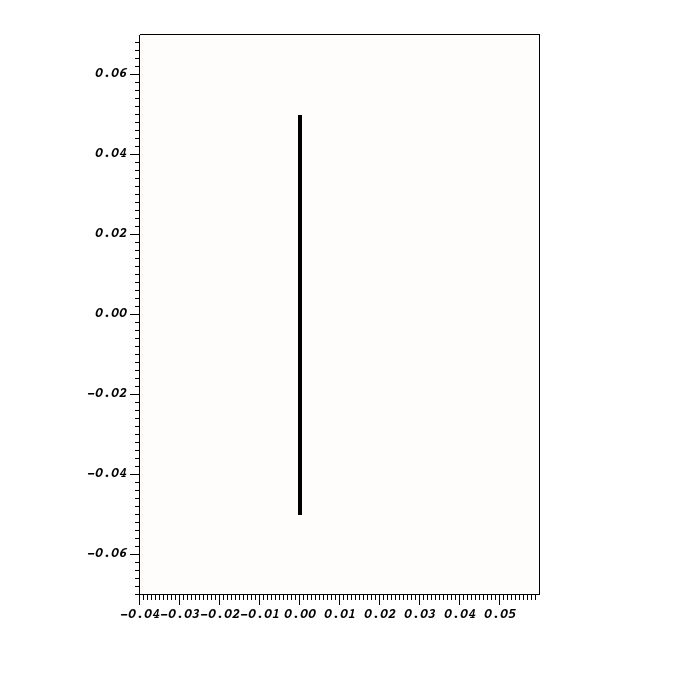
\includegraphics[height=0.62\textheight]{ch6-leaf-mesh-t0.png}\hspace{6mm}
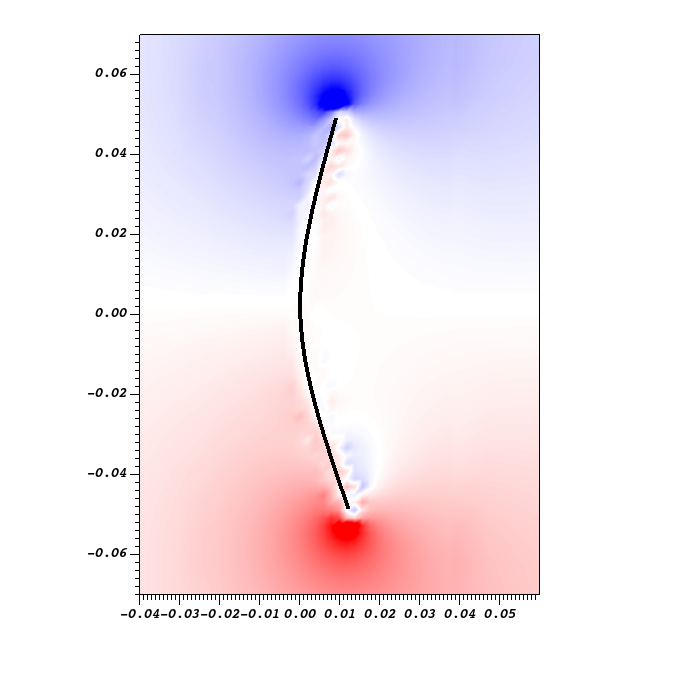
\includegraphics[height=0.62\textheight]{ch6-leaf-mesh-t2.png}\\
{\small The leaf of IB/03 as VisIt draws it from \code{lag\_data.visit}: the \code{.spring} file as lines, at $t = 0$ and $t = 2$ s, over the vorticity (IBAMR 0.19.0).}
\end{frame}

% 35b
\begin{frame}{The structure in VisIt: what is drawn}
\begin{itemize}
  \item IBAMR's Silo writer (\code{LSiloDataWriter}) turns the structure into a mesh named \code{<name>\_mesh}: the points are the vertices, and the \al{springs and crosslink springs are its edges}. Beams, targets, anchors and masses are not drawn.
  \item So a structure without springs appears as unconnected points, and a band with a missing closing spring shows its gap.
  \item The positions written are the current ones, every \code{viz\_dump\_interval} steps, so the mesh moves with the structure; VisIt's time slider steps through the frames. The leaf's bend at $t = 2$ s above is the \code{.spring} lines following the points.
  \item The same writer gives each structure its own mesh, so two plates (IB/07) are two meshes, \code{plate2d\_left\_512\_mesh} and \code{plate2d\_rght\_512\_mesh}, which you add as two plots.
  \item Chapter 26 does this in the GUI; chapter 28 adds the finite element meshes of IBFE, which are written differently (ExodusII).
\end{itemize}
\end{frame}

% 36
\begin{frame}{Structures built in the program instead of in files}
\begin{itemize}
  \item \code{IBStandardInitializer} is a thin layer over \code{IBRedundantInitializer}, which lets \code{main.cpp} \al{generate the points and elements in C++} through callback functions (\code{registerInitStructureFunction}, \code{registerInitSpringDataFunction}, and the same for beams, targets, rods and the rest), without any files.
  \item IBAMR's own \code{IB/explicit/ex0} does this; so do \code{adv\_diff/ex6}, \code{ex7} and the \code{IBLevelSet} examples (0.19.0).
  \item When it pays: parametric studies where the structure changes with an input parameter (no file to regenerate), structures of millions of points (no file to read on every process), and structures that depend on the grid at run time.
  \item When it does not: anything you want to look at, share or regenerate without a compiler. Files are easier to inspect, version and plot, and every example in this series uses them.
\end{itemize}
\vspace{2mm}
\begin{punchbox}
\small The same \code{IBStandardInitializer} block still names the structure and its level; only the data source changes. Chapter 15 walks through \code{ex0}'s callbacks next to the file version of the same shape.
\end{punchbox}
\end{frame}

% 37
\begin{frame}{IB2d's files, side by side}
\scriptsize
\begin{tabular}{@{}L{0.09\textwidth}L{0.38\textwidth}L{0.42\textwidth}@{}}
\toprule
File & IBAMR & IB2d\\
\midrule
\code{.vertex} & count, then \code{x y} per line; index = line number from \al{0} & the same, but the index counts from \al{1}\\
\code{.spring} & \code{i j kappa L [fcn [params]]} & \code{master slave k L [alpha]}, with an optional nonlinearity exponent \code{alpha}\\
\code{.beam} & \code{i j k kappa [Cx Cy]}: a curvature \emph{vector} & \code{i j k k\_beam C}: a scalar curvature; IB2d also has \code{.nonInv\_beam} (non-invariant beams)\\
\code{.target} & \code{i kappa [eta]} & \code{ID k\_target}\\
\code{.mass} & \code{i mass kappa} & \code{ID mass k\_mass}\\
others & \code{.xspring}, \code{.anchor}, \code{.rod}, \code{.director}, \code{.inst}, \code{.source} & \code{.muscle}, \code{.porous}, \code{.concentration}, \code{.geo\_connect}, \ldots\\
\bottomrule
\end{tabular}
\vspace{2mm}
\small
\begin{itemize}
  \item The geometry is the same: a structure generated for IB2d runs in IBAMR after the indices are shifted by one and the beam curvature is turned into a vector (and the units checked: IB2d's examples are usually dimensionless).
  \item MeshmerizeMe (chapter 4f) writes IB2d files from a drawing; Part II, chapter 4a, is the IB2d counterpart of this chapter and gives IB2d's full list.
\end{itemize}
\sourcecredit{IB2d formats from the IB2d repository's rubber-band example and generators (\url{https://github.com/nickabattista/IB2d}).}
\end{frame}

% 38
\begin{frame}{Reading an example folder}
\scriptsize
\begin{tabular}{@{}L{0.3\textwidth}L{0.62\textwidth}@{}}
\toprule
In \code{examples/IB/03-tethered-beam/} & What it is\\
\midrule
\code{leaf\_512.vertex} & 103 lines after the count: the leaf's points, top to bottom\\
\code{leaf\_512.spring} & 102 springs: \code{0 1 3.0600e+04 9.8039e-04}, \ldots, with $K/\Delta s$ for $K = 30$ N and $L = \Delta s$\\
\code{leaf\_512.beam} & 101 beams: \code{0 1 2 5.3060e+06}, \ldots, with $EI/\Delta s^3$ for $EI = 5\times10^{-3}$ N\,m$^2$, no curvature\\
\code{leaf\_512.target} & 2 lines: points 50 and 51 with $3.06\times10^4$, no damping\\
\code{generate\_mesh2d.m}, \code{.py} & the scripts that wrote the four files; change \code{N}, \code{kappa\_spring}, \code{kappa\_beam} or \code{plate\_length} here\\
\code{input2d} & \code{structure\_names = "leaf\_512"} and \code{level\_number = MAX\_LEVELS - 1}; the rest of the physics\\
\code{main.cpp} & the rubber band's program: it never mentions the files\\
\code{README.md} & what the numbers above mean and what the run shows\\
\bottomrule
\end{tabular}
\vspace{2mm}
\begin{punchbox}
\small Every example folder in this series reads this way. The \code{512} in the names is the finest grid count the files were made for; regenerate with another \code{N} and the names change with it, so that files for different grids never mix.
\end{punchbox}
\end{frame}

% 39
\begin{frame}{Homework: your own rubber band}
\begin{columns}[T,onlytextwidth]
\begin{column}{0.55\textwidth}
From the 2018 and 2020 courses (Appendix C collects the full set):
\begin{enumerate}
  \item Copy IB/01 and write your own generator, in any language, that puts down the \code{.vertex} points and the \code{.spring} springs of a rubber band.
  \item Make the band \al{50\% smaller} and deform it initially in a different way (an ellipse the other way, a square, a band with a dent).
  \item Run it and look at it in VisIt. The 2018 version asked for two screenshots of the band oscillating; the 2020 version for the generator and the pictures in a shared folder.
\end{enumerate}
\end{column}
\begin{column}{0.43\textwidth}
\begin{punchbox}
\small What to check in your files before running: the count equals the number of lines minus one; the indices run from 0; the ring is closed; the spacing is about $\Delta x/2$; the stiffness in the file is $K/\Delta s$ for the $K$ you chose. Then a short run and the log's ``read N'' lines.
\end{punchbox}
\vspace{2mm}
\small Extension: add a \code{.beam} file to the band (IB/03's generator shows the loop) and watch the dent smooth out faster.
\end{column}
\end{columns}
\end{frame}

% 40
\begin{frame}{Rules of thumb}
\scriptsize
\begin{tabular}{@{}L{0.26\textwidth}L{0.66\textwidth}@{}}
\toprule
Rule & Why\\
\midrule
One generator per structure, kept with the files & the files are derived data; the constants and the geometry live in the script (slide 28)\\
Indices from 0, local to the structure & IBAMR's convention; \code{.xspring} is the only file with global indices (slide 8)\\
Write every column that matters, even when a default would do & the rest length is required anyway; a stated 0 is clearer than a missing value (slide 11)\\
Stiffnesses as $K/\Delta s$ and $EI/\Delta s^3$ & so that the physics does not change when you refine (slide 15)\\
Point spacing about $\Delta x/2$ & chapter 5; the generators compute it from $N$\\
Closed curves have as many springs as points & the closing spring (slide 12)\\
Read the log's ``read N'' lines after every change & missing files are skipped silently (slide 25)\\
A short run, then VisIt, then the long run & every file error appears before step 1 (slides 26, 34)\\
Unix line endings everywhere & the structure files tolerate CRLF, the input file does not (slide 23)\\
\bottomrule
\end{tabular}
\end{frame}

% 41
\begin{frame}{Summary}
\small
\begin{enumerate}
  \item A structure is a \code{.vertex} file (required) plus elastic elements in \code{.spring}, \code{.beam}, \code{.target} and, less often, \code{.xspring}, \code{.anchor}, \code{.mass}, \code{.rod}/\code{.director}, \code{.inst} and \code{.source}; the input file names the structure and its grid level.
  \item Points are numbered from 0 by their line in the \code{.vertex} file; springs join pairs, beams act on triples through their middle point, targets tether single points to a position that the program may move.
  \item The file stiffnesses are $K/\Delta s$ and $EI/\Delta s^3$, so they are rescaled by the generator when the grid changes; the rest length of a spring is required, whatever the header says.
  \item The log reports what was read and what was skipped; the reader stops with a precise line number for malformed files but says nothing about a missing optional file or a missing closing spring.
  \item Generate, count, plot, run a few steps, look in VisIt, then run.
\end{enumerate}
\vspace{2mm}
\begin{homebox}
\small Next, chapter 7: boundary conditions and the set-up of the fluid box, where the input file's other half is explained.
\end{homebox}
\end{frame}

% 42
\begin{frame}{What changed since the older course notes}
\small
\begin{itemize}
  \item The format table now covers every file the 0.19.0 initializer reads, including \code{.xspring}, \code{.anchor}, \code{.rod}, \code{.director}, \code{.inst} and \code{.source}, which the 2013--2020 lectures listed partly or not at all, and the \code{uniform\_*}, \code{enable\_*}, \code{posn\_shift}, \code{length\_scale\_factor} and \code{use\_file\_batons} keys.
  \item The rest-length statement is corrected: required, not optional (tested), against the header comment that the 2020 lecture quoted.
  \item The units of the file stiffnesses are stated for the first time ($K/\Delta s$, $EI/\Delta s^3$), with the derivation.
  \item The comment, line-ending and number rules are tested rather than assumed, and the error messages are quoted from runs.
  \item The closing-spring bug of the UNC generator (643 springs for 644 points) is explained and fixed in IB/01's generator; the generator excerpts are IB/01's current ones, with a Python version.
  \item The log's ``read N'' and ``skipping read'' lines and the zero-stiffness warnings are new material.
  \item The resources slide is updated: the Google Code links of 2015 and the class-documentation link of 2020 are dead; the header file is the format reference.
  \item IB2d's formats are compared in one table; the IB2d chapter (4a) keeps the full list.
\end{itemize}
\end{frame}

% 43
\begin{frame}{References}
\scriptsize
\begin{itemize}
  \item IBAMR source, version 0.19.0: \code{include/ibamr/IBStandardInitializer.h} (the file-format comments), \code{src/IB/IBStandardInitializer.cpp} (the readers), \code{src/IB/IBStandardForceGen.cpp} and \code{include/ibamr/IBSpringForceFunctions.h} (the forces), \code{src/IB/IBRedundantInitializer.cpp} (structures from code). \url{https://github.com/IBAMR/IBAMR}
  \item IBAMR documentation index: \url{https://ibamr.github.io/docs}; wiki and FAQ: \url{https://github.com/IBAMR/IBAMR/wiki}; users' group: \url{https://groups.google.com/g/ibamr-users}; discussions: \url{https://github.com/IBAMR/IBAMR/discussions}.
  \item C. S. Peskin. The immersed boundary method. \emph{Acta Numerica} 11:479--517, 2002. \url{https://math.nyu.edu/~peskin/}
  \item N. A. Battista, W. C. Strickland and L. A. Miller. IB2d: a Python and MATLAB implementation of the immersed boundary method. \emph{Bioinspiration \& Biomimetics} 12:036003, 2017. \url{https://github.com/nickabattista/IB2d}
  \item D. M. Senter et al. A semi-automated finite difference mesh creation method for use with immersed boundary software IB2d and IBAMR. \emph{Bioinspiration \& Biomimetics} 16:016008, 2021.
  \item The tests behind slides 23 and 26: \code{wsl/final/ch6\_errors.sh} in the working folder of these notes, run with IBAMR 0.19.0 on the rubber band of IB/01.
  \item Sources: \emph{IBAMR Tutorial: Getting Started} (2013--2021); \emph{MATH 769 Lecture 5: IBAMR Input Files} (2015); \emph{3 -- IBAMR Associated Files} (2018--2019); \emph{IBAMR Lecture 3} (2020, edited 2024); the lab's 2012 ReadMe and 2013 input-visualization decks.
\end{itemize}
\end{frame}

\end{document}
